\label{chapt:intro}

Living in the era where it is nearly impossible to live without it, cellular service is very important. Up nearly 13\% from last year, it is said that US consumers are checking their mobile devices at a remarkable rate of 9 billion times per day \cite{deloittestat}.\\

It is numbers like these that have inspired \Company to begin research and development of the worlds first commercial, autonomous, aerostat's. Led by state of the art controls, Altaeros' mission is to help provide these services, including power in even the most remote of areas. The latest product is seen below in Figure~\ref{fig:1_companypic}~\cite{companypicweb}.

\begin{figure}[H]
	\centering
	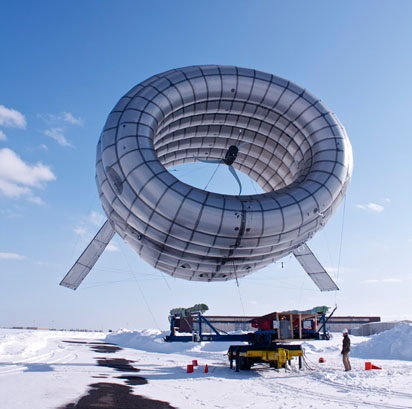
\includegraphics[width=0.6\textwidth]{1_companypic}
	\caption{Overview of Altaeros' aerostat.}\protect\cite{companypicweb}
	\label{fig:1_companypic}
\end{figure}


The above figure raises the question, how does this system remain stable. This is achieved through the system's tether management system.

\section{Background} % (fold)

The winch system is responible for the control of the aerostat. An overview of similar system used by Altaeros is shown below in Figure~\ref{fig:1_winch}~\cite{winchpic}.
\begin{figure}[H]
	\centering
	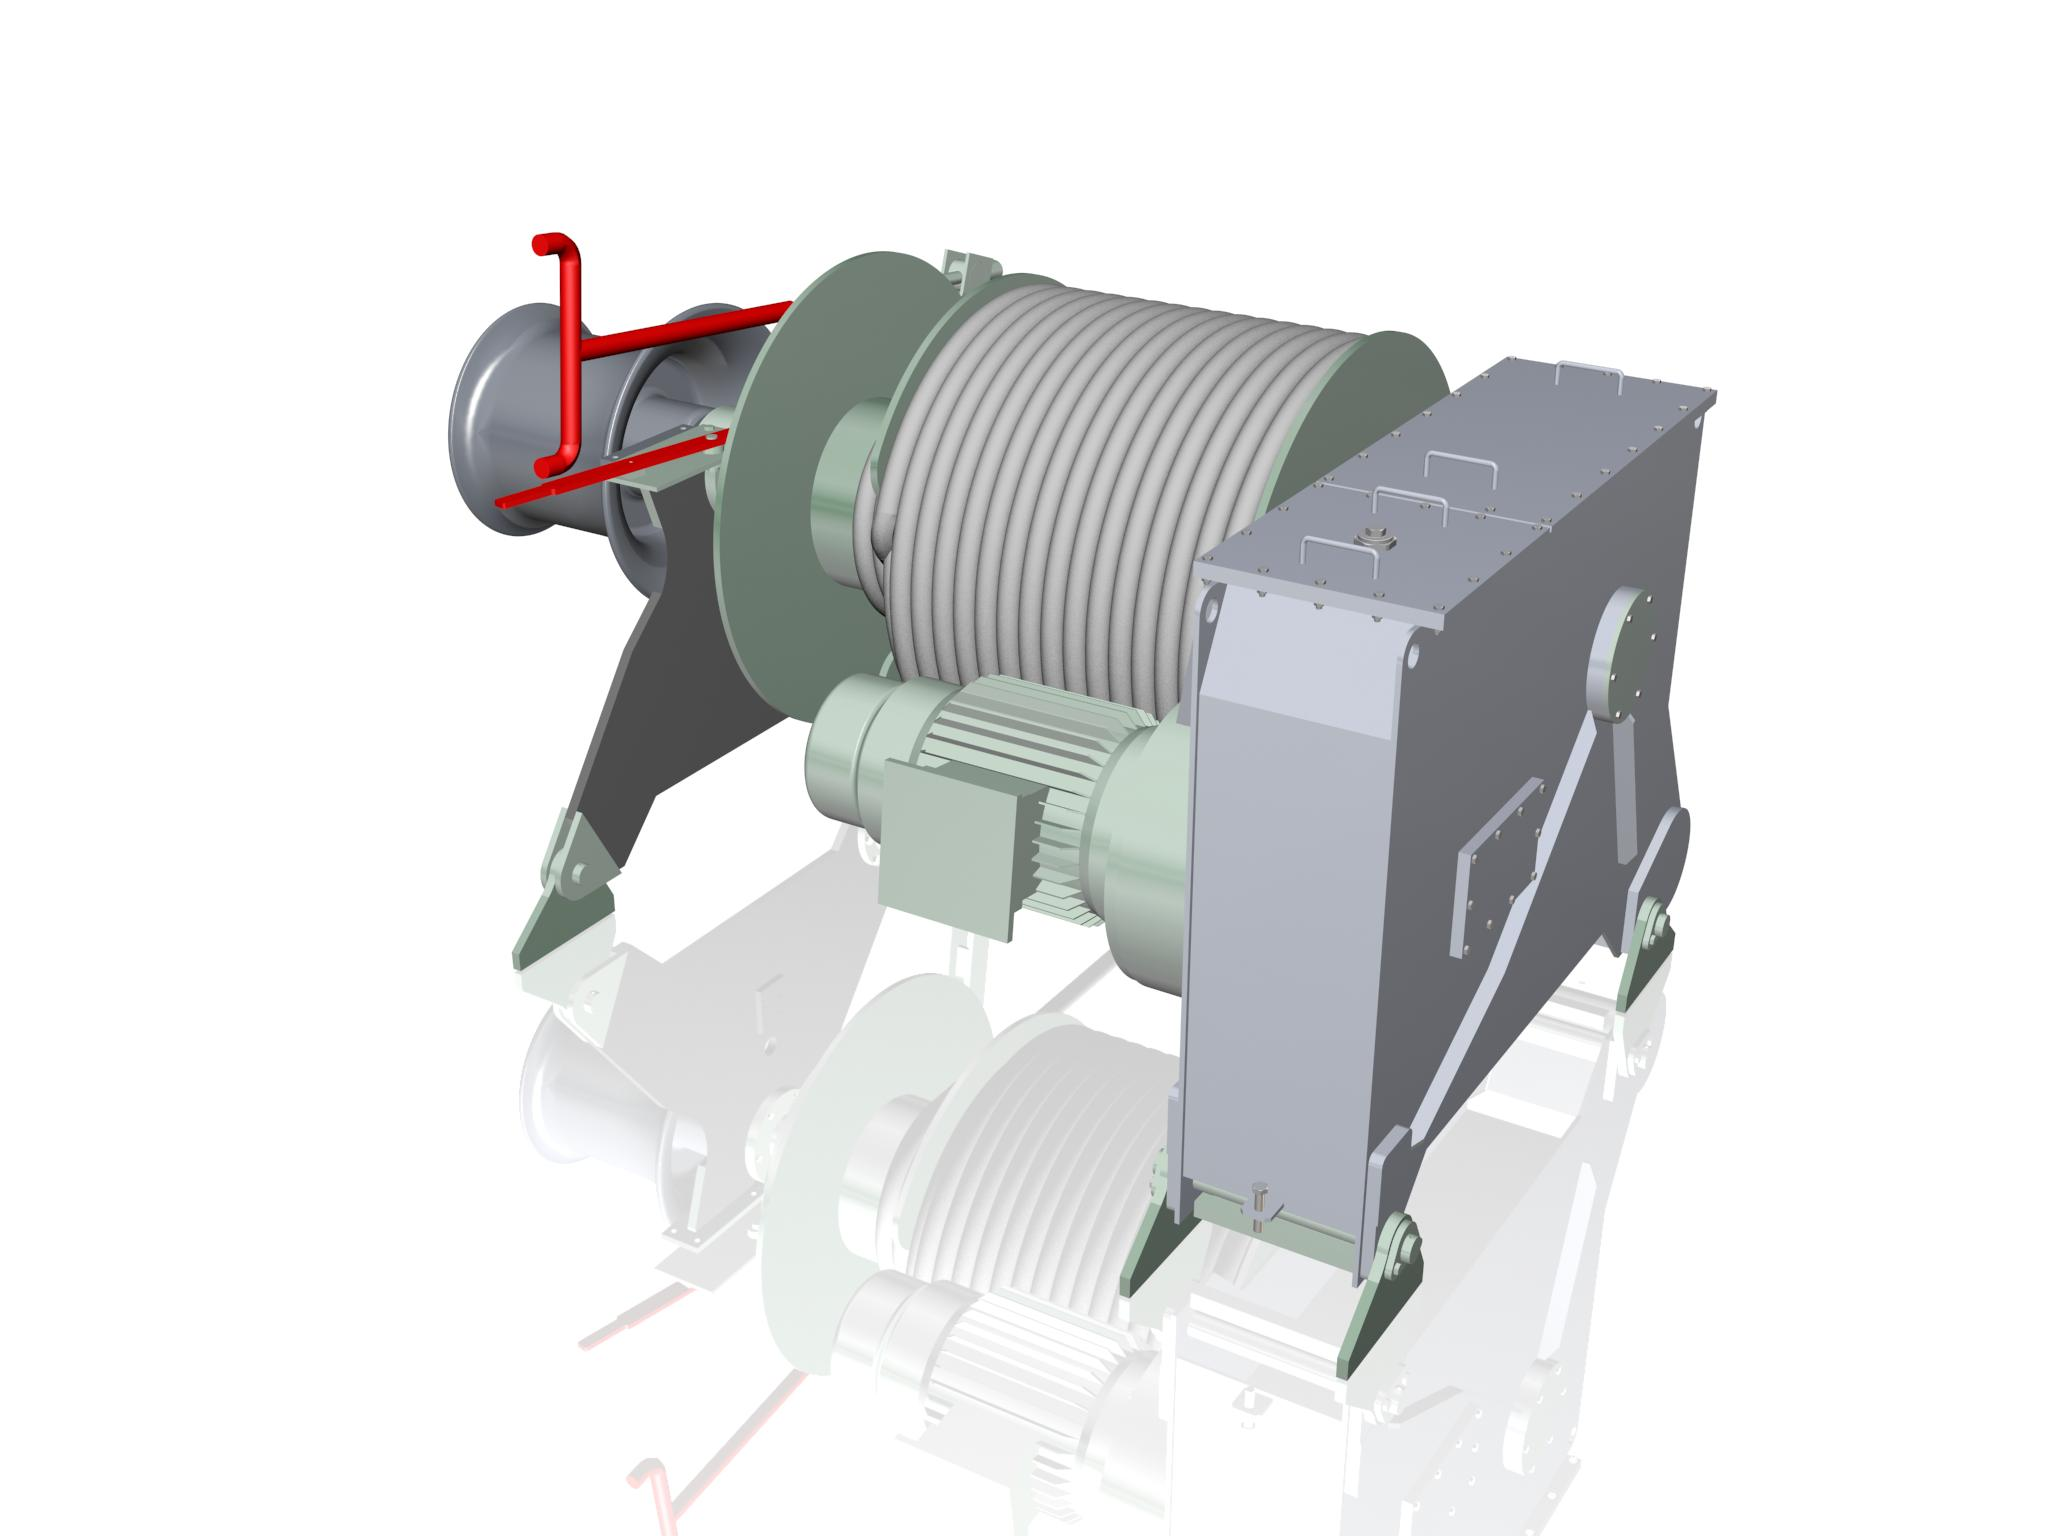
\includegraphics[scale=0.2]{1_winch}
	%% must use protect to put reference in caption
	\caption{Example of common winch system.}\protect\cite{winchpic}
	\label{fig:1_winch}
\end{figure}

It has been deemed that Altaeros could manufacture a more custom, cheaper and efficient winch system. In order to assure that the system is capable of handling the large aerodynamic loads translated by the tether, a complete structural analysis must be completed.

\section{Purpose}
The purpose of this report is to perform the structural analysis in order to assure that the winch drum assembly is capable of handling the large loads.\\

An overview of the winches drum assembly is shown from the 3D computer aided design (CAD) model developed with Inventor \cite{INVENTOR} as per Figure~\ref{fig:1_drum}.
\begin{figure}[H]
	\centering
	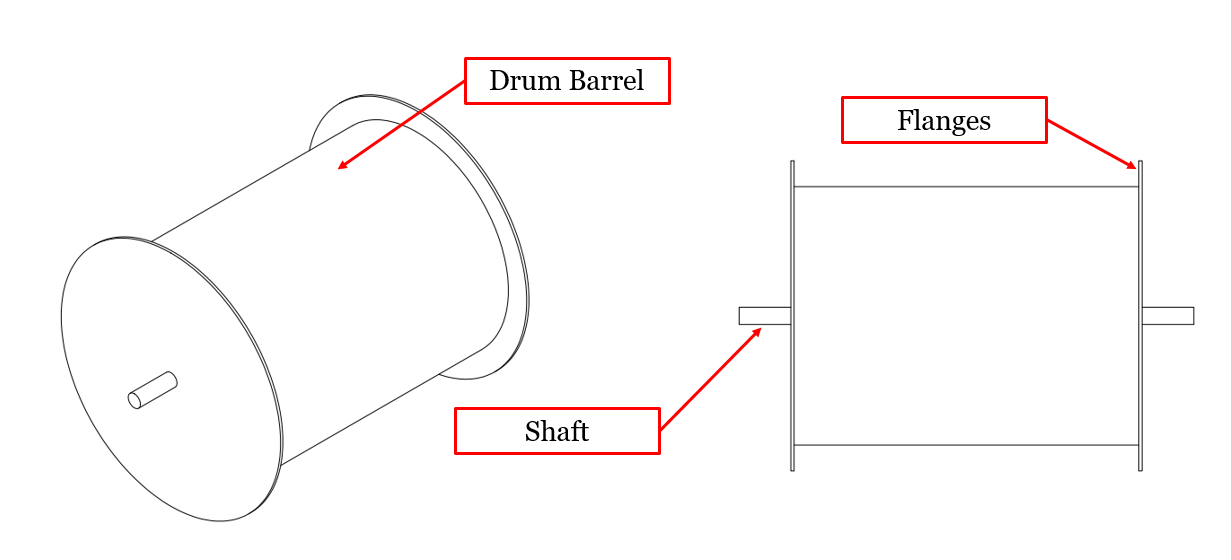
\includegraphics[scale=0.5]{1_drum}
	\caption{Drum assembly CAD model.}
	\label{fig:1_drum}
\end{figure}

It is important to realize that most of loading from the tether will be translated as pressure onto the barrel. This loading scenario will be investigated to properly size the winch barrel thicknesses which is the driving design dimension.

\section{Scope}

In the following sections of this report, the relevant parameters will be presented. From this, existing codes and standards will be investigated in exploring what a quick analysis would yield. From this, a more advanced numerical approach will be presented. These results will then be validated by use of finite element analysis (FEA). Finally, all results will be discussed, relevant conclusions and recommendations will be made.